\documentclass[tikz]{standalone}
\begin{document}
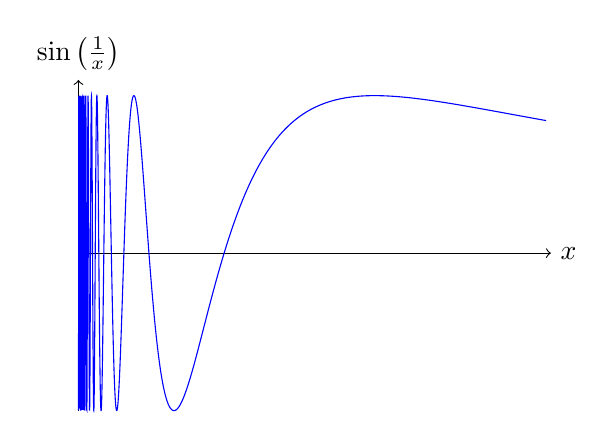
\begin{tikzpicture}[x=3cm, scale=2]
  % \draw[xstep=.2,ystep=.5,lightgray,ultra thin] (-0.1,-1.5) grid
  % (.7,1.5);
  \draw[->] (0,0) -- (1,0) node[right] {$x$};
  \draw[->] (0,-1) -- (0,1.1) node[above] {$\sin \left( \frac{1}{x} \right)$};
  \draw[blue,domain=0.01:1,samples=9100] plot (\x-.01, {sin((1/\x)r)});
  % \clip (0,-1) rectangle (1,1);
\end{tikzpicture}
\end{document}
